\newpage
\section{\acrlong{ser}}
To achieve Emotion Recognition through speech, we will follow two approaches: 
\begin{enumerate}
    \item using \emph{phonological} information (pitch, amplitude, spectral features, etc.)
    \item using \emph{semantic} information (words, grammar)
\end{enumerate}

\vspace{5mm}
% Jana's task:
%\emph{1. Approach: phonological information}

\noindent For the first approach, we will create a \acrfull{crnn},  i.e. a sequential neural network with 1D convolutional layers. It will take the spectrograms as input that we obtained through preprocessing and outputs the most likely emotion associated with the input. Here, the python library Keras can be used to easily build a neural network by adding desired layers to the model. Keras is open-source and available for free. \\

%\noindent \emph{2. Approach: semantic information}
\noindent For the second approach, a combination of two neural networks will be used. First, an \acrfull{asr} model transforms the spectrograms into a textual representation of the utterance. This can again be done with Keras as it additionally offers APIs to pre-trained ASR models like DeepSpeech, an open-source model by Mozilla.
Then, the obtained text is assigned to an emotion by a transformer-based neural network. Here, the python library Hugging Face can be used. It is free, open-source and offers pre-trained transformer models like BERT. 
Since the ASR model and the transformer model are already pre-trained on a large corpus of data and our application scenario is kept general instead of domain-specific, it is not strictly necessary to find additional datasets for training the ASR model and the transformer model ourselves. \\

\begin{figure}[h!]
\centering
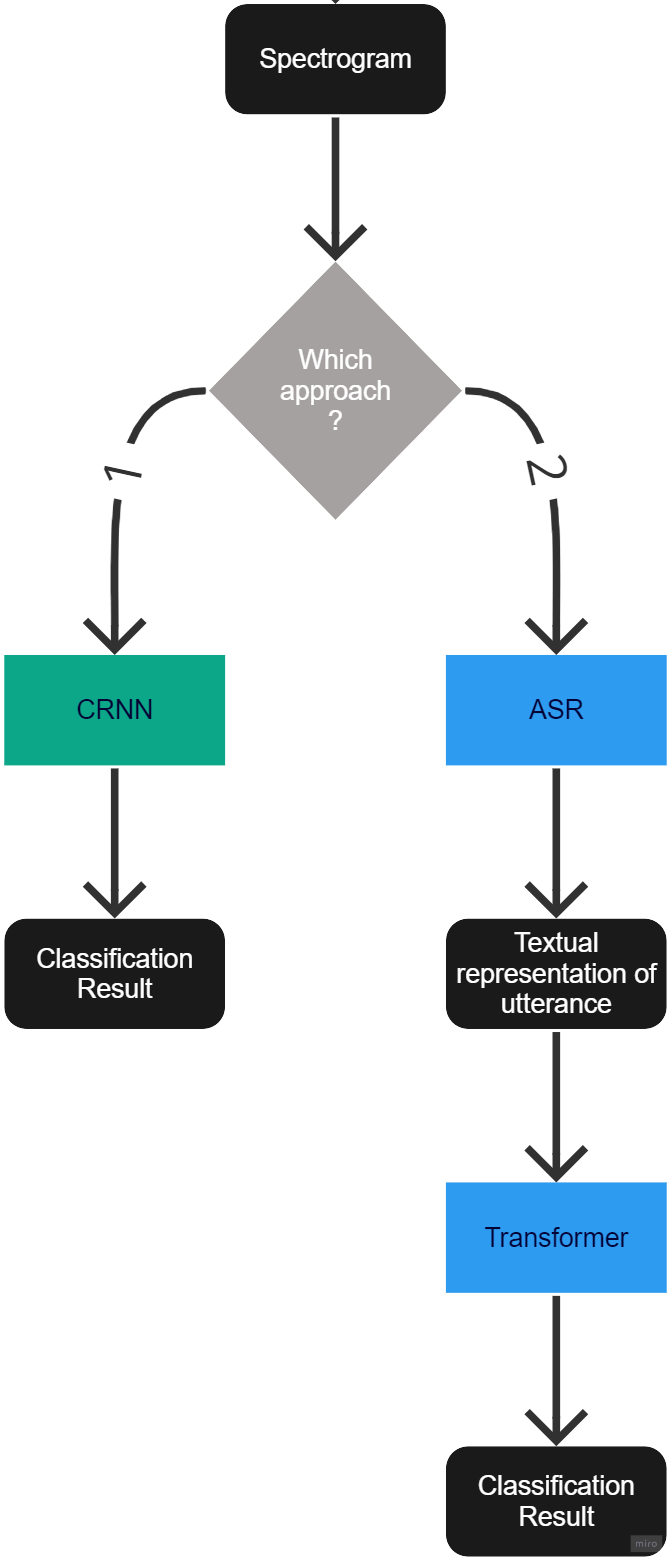
\includegraphics[scale=0.6]{images/SER_Modeling.png}\\
\caption{\acrshort{ser} Modeling.}\label{fig:ser_modeling}
\end{figure}
